\documentclass[11pt,letterpaper]{article}
\usepackage{samstyle}

\title{
        Pueblo Farida}
        
\author{
	Profesor\\
	Sergio Andres Monsalve Castañeda\\
	smonsal3@eafit.edu.co
}

\begin{document}
 
\pagestyle{fancyplain}
\fancyhf{}
\headheight=20pt %para cambiar el tamaño del encabezado
\renewcommand{\headrulewidth}{0pt} %espesor del encabezado

% \lhead %la "L" indica a la izquierda
% {
% }

\fancyfoot[c]{\thepage}

\maketitle

\begin{minipage}{3cm}
% 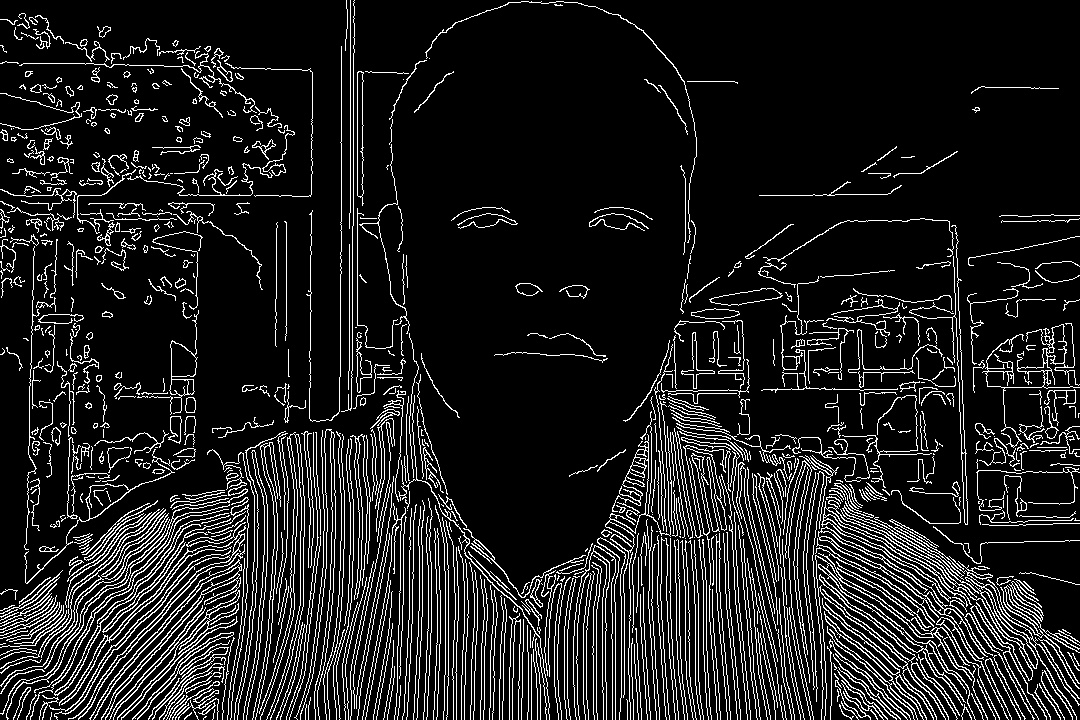
\includegraphics[width=15cm]{aux/SamCanny.jpg}
\end{minipage}


\section{Descripción}

En el camino a un pueblo había una serie de magos que se encargaban de dar monedas de oro a quienes pasaban por el camino bajo una condición.

Si pasabas al lado de un mago le podias pedir monedas si y solo si a el mago anterior no le habias pedido.

Y te podias quedar con las monedas si recolectabas la  maxima  cantidad posible de monedas segun los magos que hubieran y el total de dinero que tenian.

\section{Objetivo}

Conociendo cuantos magos hay y cuantas monedas tiene cada uno calcule el maximo numero de monedas que puede recolectar en camino al pueblo. 


\section{Entrada}

la primera linea contiene el numero de casos a analizar. Cada caso comienza con un numero M de Magos que hay camino al publo. $0 <= N <= 10**4$. La siguiente sdlinea es el numero de monedas que cada Mago tiene $0 <= C <= 10**9$ y estos estan descritos en el orden que se les puede encontrar de camino al pueblo


\section{Salida}

Para cada caso de prueba imprima: ``Caso c: X'' sin comillas, donde c es el numero del caso comenzando en 1 y x es el numero máximo de monedas que se pueden obtener.

\section{Ejemplo}
\subsection{Entrada}
\lstinputlisting{Farida.in}
\subsection{Salida}
\lstinputlisting{Farida.ot}

%\bibliographystyle{plainnat}
%\bibliography{refs}

\end{document}


